%************************************************
% IMPLEMENTATION
%************************************************

\chapter{Implementation} \label{chap: implementation}

\paragraph{} \textit{In this chapter we present the tools that have been used for the implementation of the project, some details about the data, the data preprocessing procedure, a description of the models' configurations and experiments conducted and the produced results.}


%----------------------------------------------------------------
% Tools
%----------------------------------------------------------------

\section{Tools} \label{sec: tools}
\paragraph{} All the computation for this project has been conducted on a university server equipped with Ubuntu SMP version 16.04.1 and a NVIDIA TITAN Xp graphics card for the deep learning training processes. A brief description of the software tools used for the project will follow.

\paragraph{Python} \cite{python} The programming language used for this project is Python v3.6. Python is a general purpose language, known for its ease of use and understanding; however, thanks to the addition of dedicated libraries for data analysis and predictive modeling, in the last few years it has become the reference and most-used language for data science.

\paragraph{Numpy} \cite{numpy} Numpy is an extremely popular and useful library for scientific computing with Python. It allows to easily handle multidimensional data through matrix representation and to perform operation between them thanks to its broadcasting functions. Numpy has been used in all the project implementation's steps to handle and manipulate the data.

\paragraph{Pandas} \cite{pandas} Pandas is an open source library which provides efficient, flexible and easy-to-use data structures and data analysis tools for Python. Pandas is built on top of Numpy library and it is suited to handle almost any kind of data, representing them in a handy tabular form. We mainly used Pandas in order to store the results from the experiments.

\paragraph{matplotlib} \cite{matplotlib} Matplotlib is a 2D plotting library and it represents one of the most common visualization tools for Python. Its \texttt{pyplot} module provides a MATLAB-like functional interface and a wide degree of customization of the generated figures. All the plots in this thesis has been generated using matplotlib library.

\paragraph{scikit-learn} \cite{scikit-learn} Scikit-learn is a well-known, simple and efficient library for data analysis and machine learning in Python. It is open-source and is built on NumPy, SciPy, and matplotlib libraries. It provides several useful tools for data preprocessing, model selection, classification, regression, clustering and dimensionality reduction. In this project, it has been heavily used for the data preprocessing and to implement the classic machine learning models.

\paragraph{XGBoost} \cite{xgboost} XGBoost is an optimized library for distributed gradient boosting, designed to be highly efficient, flexible and portable. It implements a tree-based gradient boosting model which has been used for the gradient boosting experiments.

\paragraph{Tensorflow \& Keras} \cite{tensorflow} \cite{keras} The framework we used in order to build deep learning models is Tensorflow v2.0. Tensorflow is one of the most popular frameworks for machine learning and deep learning; it is open-source and it provides a flexible ecosystem of tools, libraries and community resources to easily build machine learning models. On top of Tensorflow, we used Keras high-level neural networks API. Keras was originally a library separated from Tensorflow, providing ready-to-use tools for fast experimentation and developing of neural networks models by running on top of TensorFlow, CNTK, or Theano. With the update to version 2.0 of Tensorflow, Keras has officially become part of Tensorflow API. We mainly used Keras library on top of Tensorflow for the implementation of deep learning models in order to generate high-level and easy-to-understand code. This choice was reasoned by the fact that this thesis project is also related to the medical field, so we tried to make the code readable also by people which are not specialized in the data scientist field.

\paragraph{Spektral} \cite{Spektral} Spektral is a Python library for graph deep learning, based on the Keras API. It provides a simple but flexible framework for creating graph neural networks (\acsp{gnn}) by making available several ready-to-use, but still highly customizable, graph-based deep learning layers. It also implements functions for the creation of a functional connectivity network from a data stream. In this project, Spektral library was used for the generation of functional connectivity graphs and for the implementation of graph-based deep learning models.


%----------------------------------------------------------------
% Data analysis
%----------------------------------------------------------------

\section{Data analysis} \label{sec: data_analysis}

\paragraph{} For this project, we were provided with 24 hours of \acs{ieeg} data generated from real measurements on a patient suffering form epilepsy. The data contains three seizures, all happening during the first three hours of recording; therefore just the data regarding the first three hours have been used in the project. The brain activity has been measured using 90 electrodes and a sampling frequency of 500 Hz, so each hour contains $1\,800\,000$ time steps of measurements.

First thing, we identified the position of the seizures in the data and their length. As already mentioned, the data contains three seizures in total, each one having a duration between $13\,000$ and $15\,000$ time steps, for a total of $42\,000$ time steps of seizure. This corresponds to 26 to 30 seconds of duration for each seizure and 84 seconds of seizure in total. Since the most important data for this project were the seizure time steps and we didn't need a huge amount of non-seizure time steps, during all the project we considered only a portion of data around each one of the three seizures, obtaining $450\,000$ time steps (15 minutes) to work with between seizure and non-seizure data in total. This should give an idea of how much limited the amount of useful data was for this project.

Some basic statistical measurements have been applied to the \acs{ieeg} data in order to familiarize with its features. The measured voltage in the \acs{ieeg} vary between about $-9\,500$ and $9\,800$ \acs{nv} (nanovolts), covering a range of about $19\,300$ \acs{nv}. Each electrode's signal oscillate through time with a standard deviation of around 82 \acs{nv} and the various electrodes signals cover different areas of the \acs{ieeg} voltage range. In Figure \ref{fig:plot_seizures} the plots of the \acs{ieeg} around the three seizures is shown. The start and end times of the seizures in each plot are indicated by red vertical lines.
\newpage
\begin{figure}[H]
    \centering
    \begin{subfigure}[t]{0.7\textwidth}
		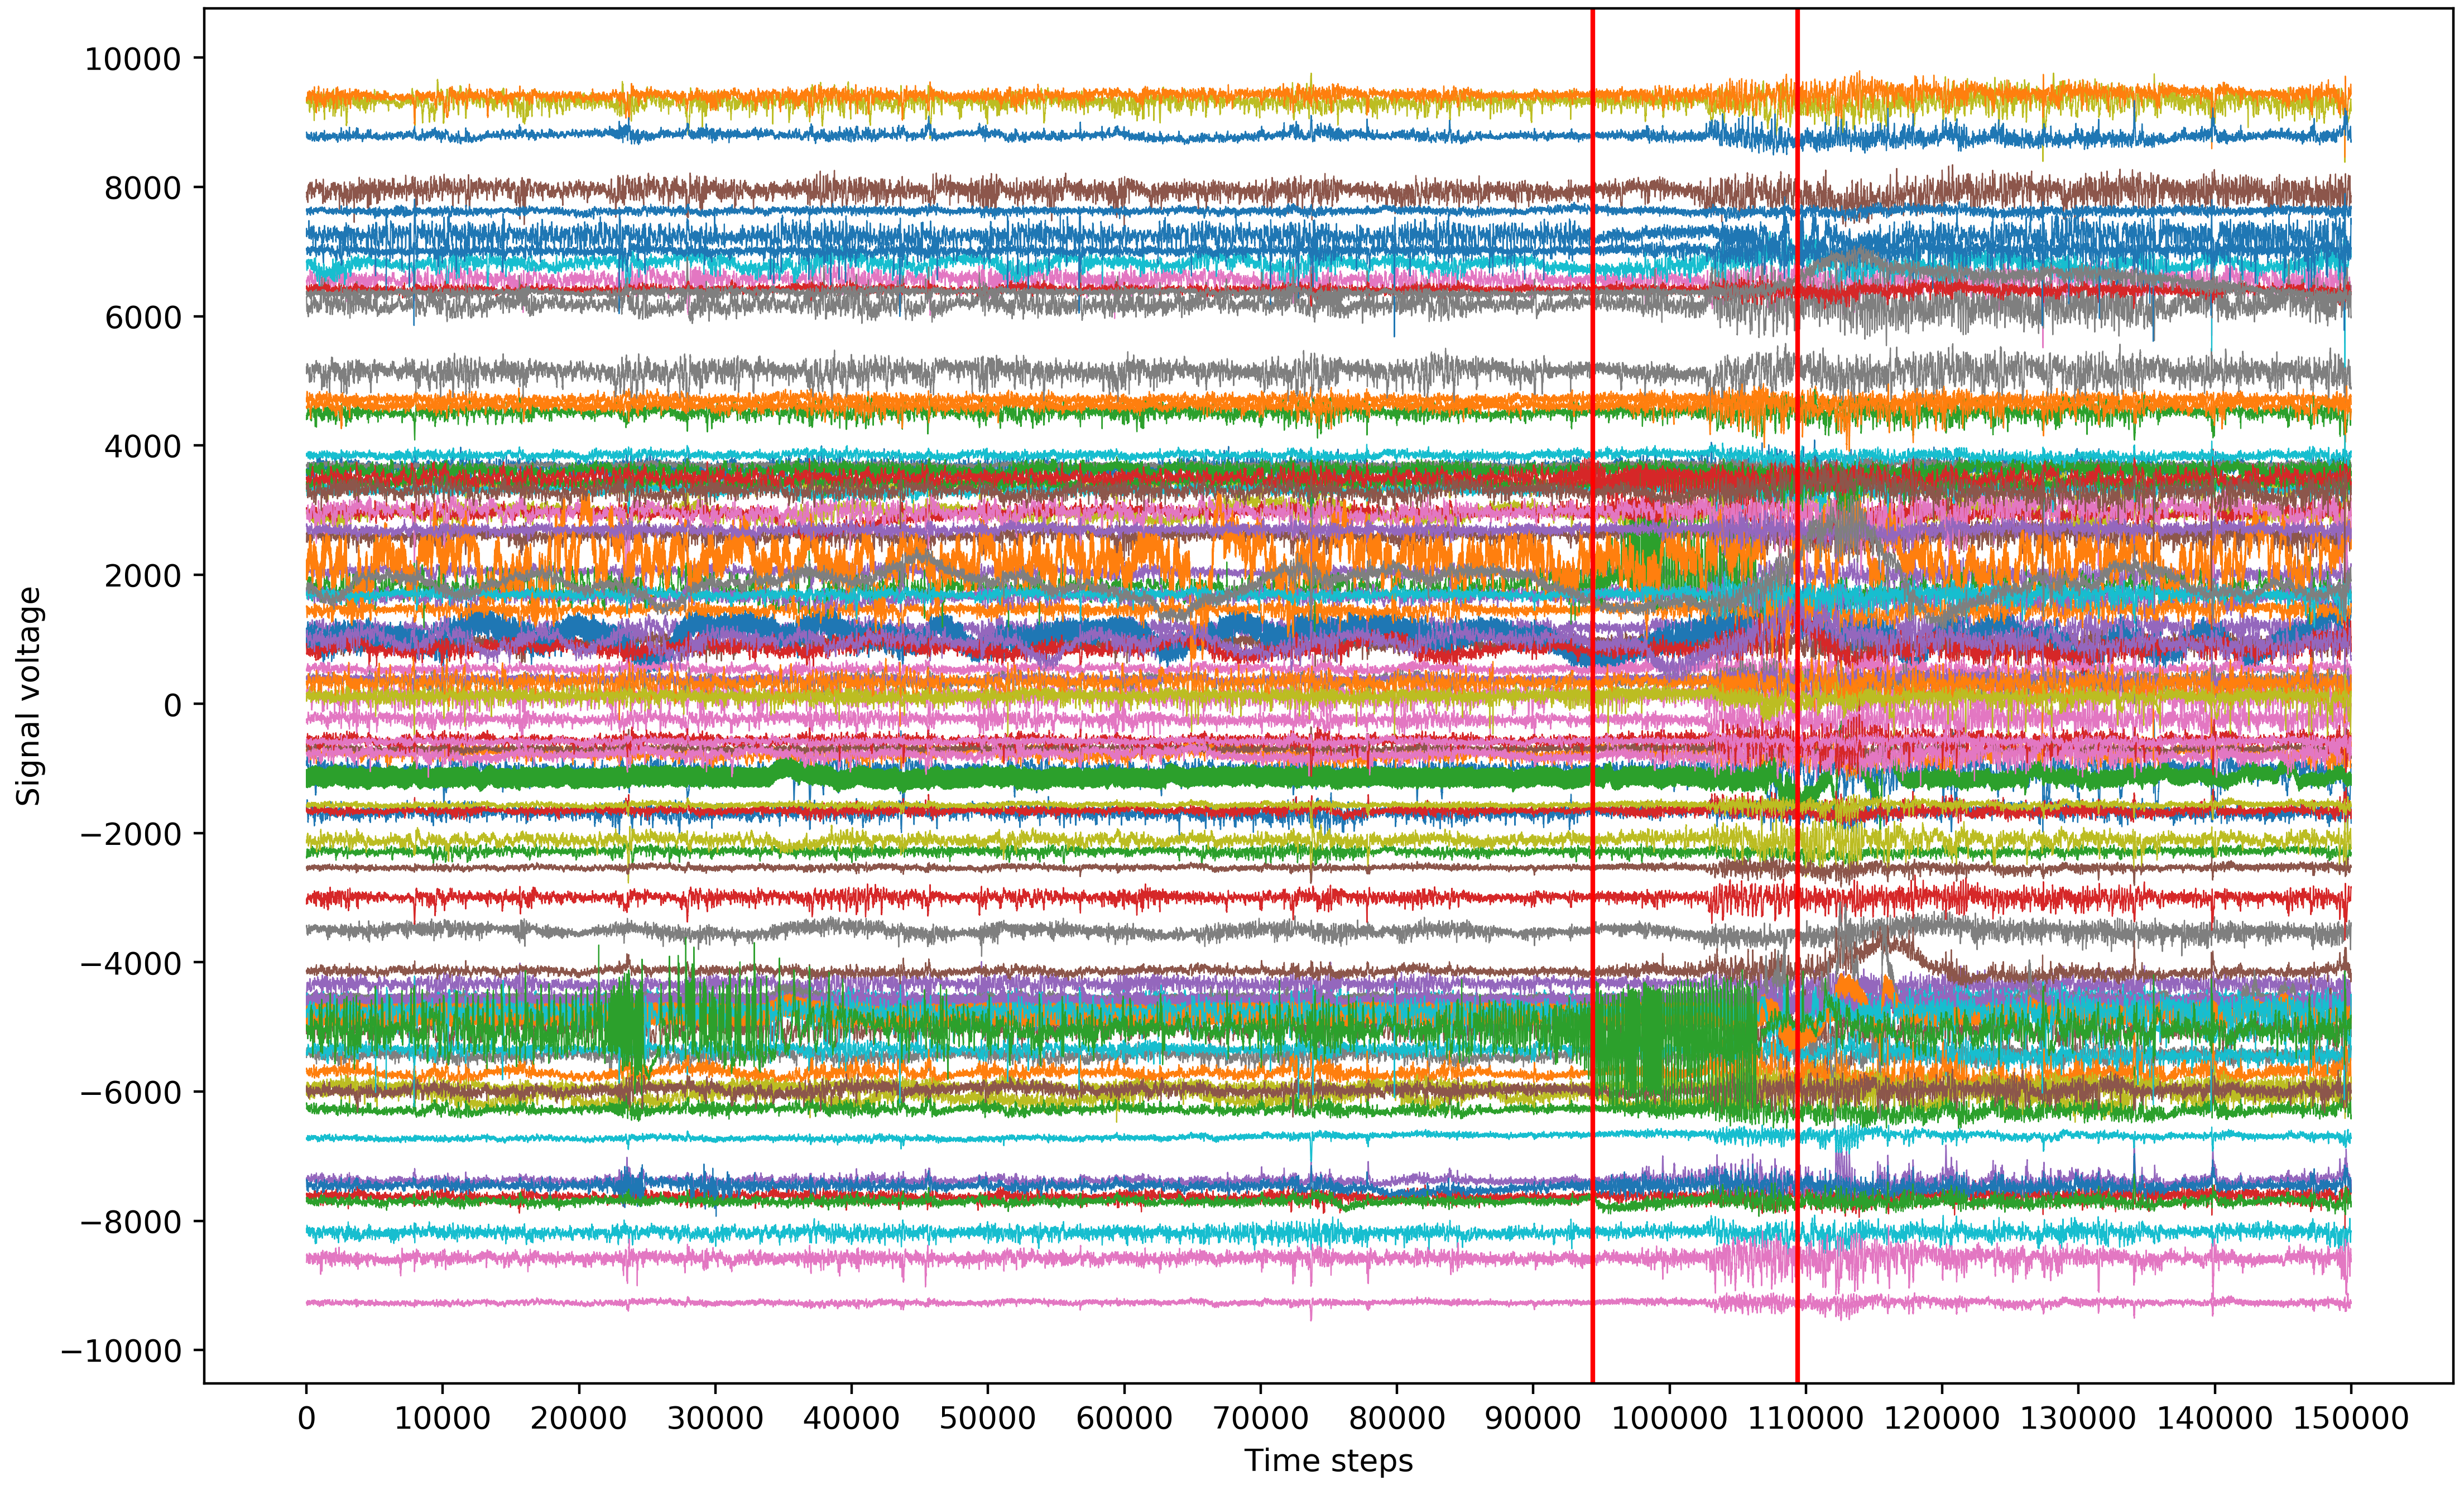
\includegraphics[width=1\textwidth]{plot_seizure1}
        \caption{First epileptic seizure}
        \label{fig:plot_seizure1}
	\end{subfigure}
	~
	\begin{subfigure}[t]{0.7\textwidth}
		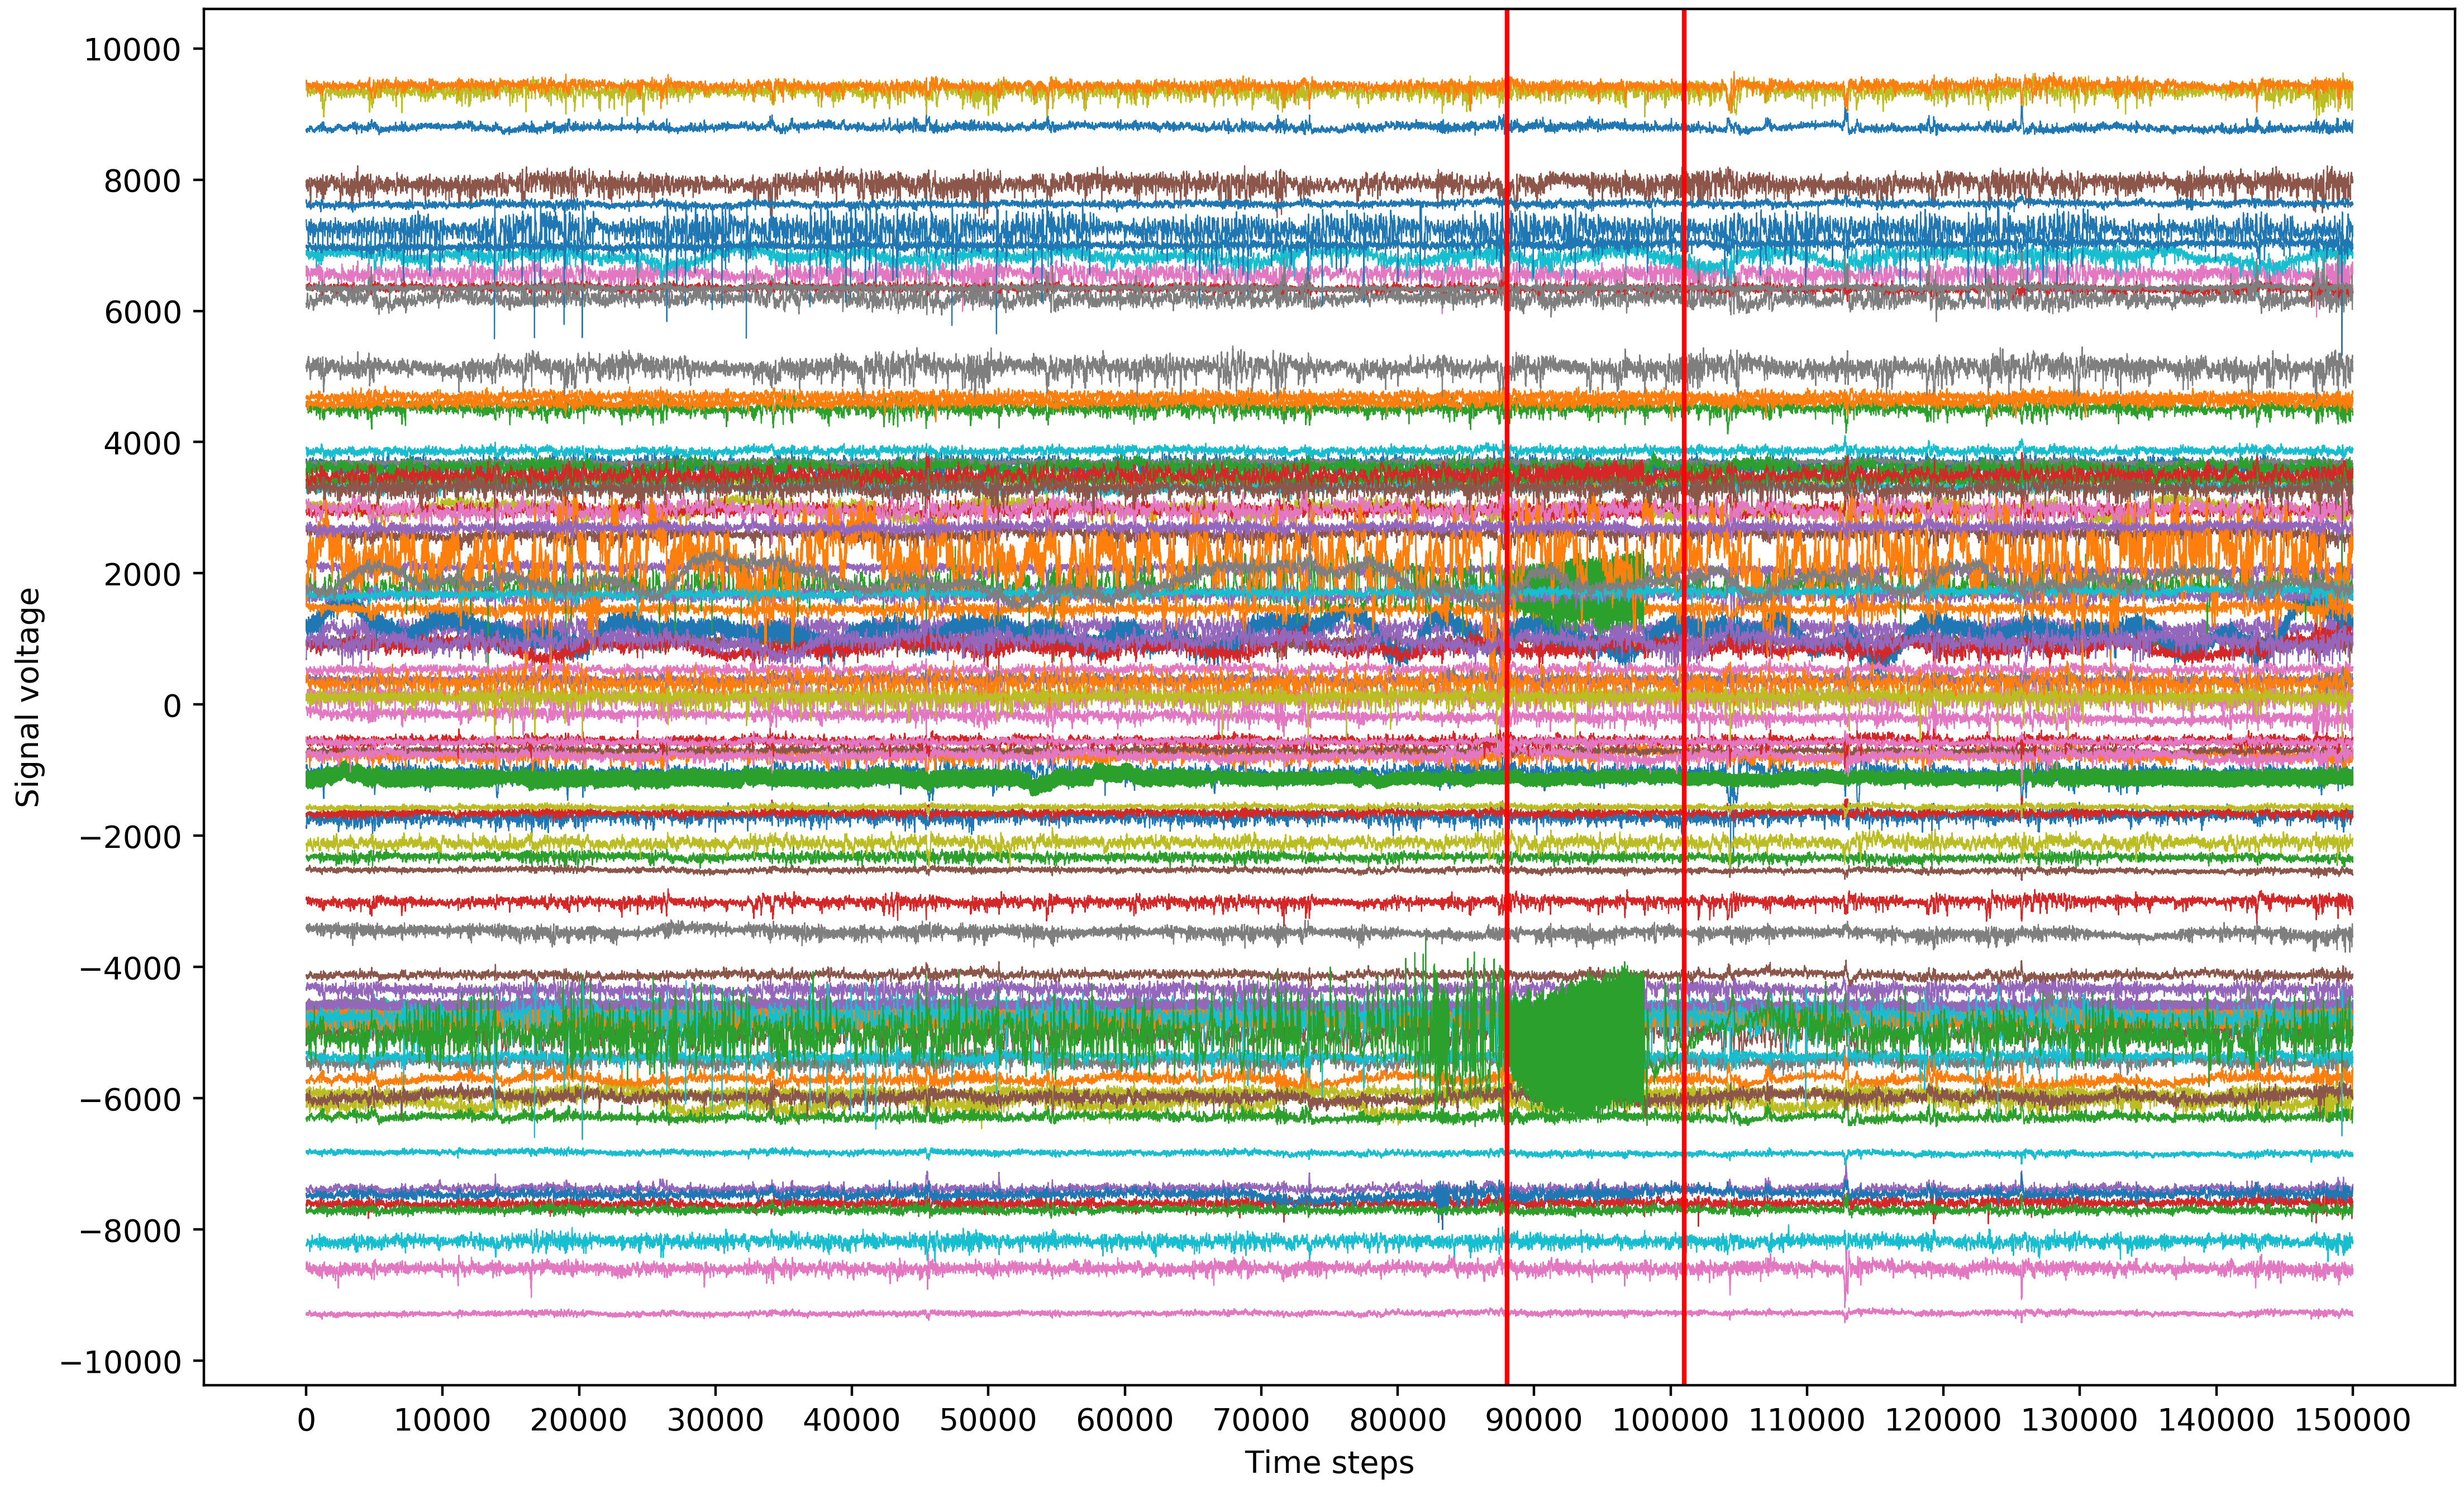
\includegraphics[width=1\textwidth]{plot_seizure2}
        \caption{Second epileptic seizure}
        \label{fig:plot_seizure2}
    \end{subfigure}
    ~
    \begin{subfigure}[t]{0.7\textwidth}
		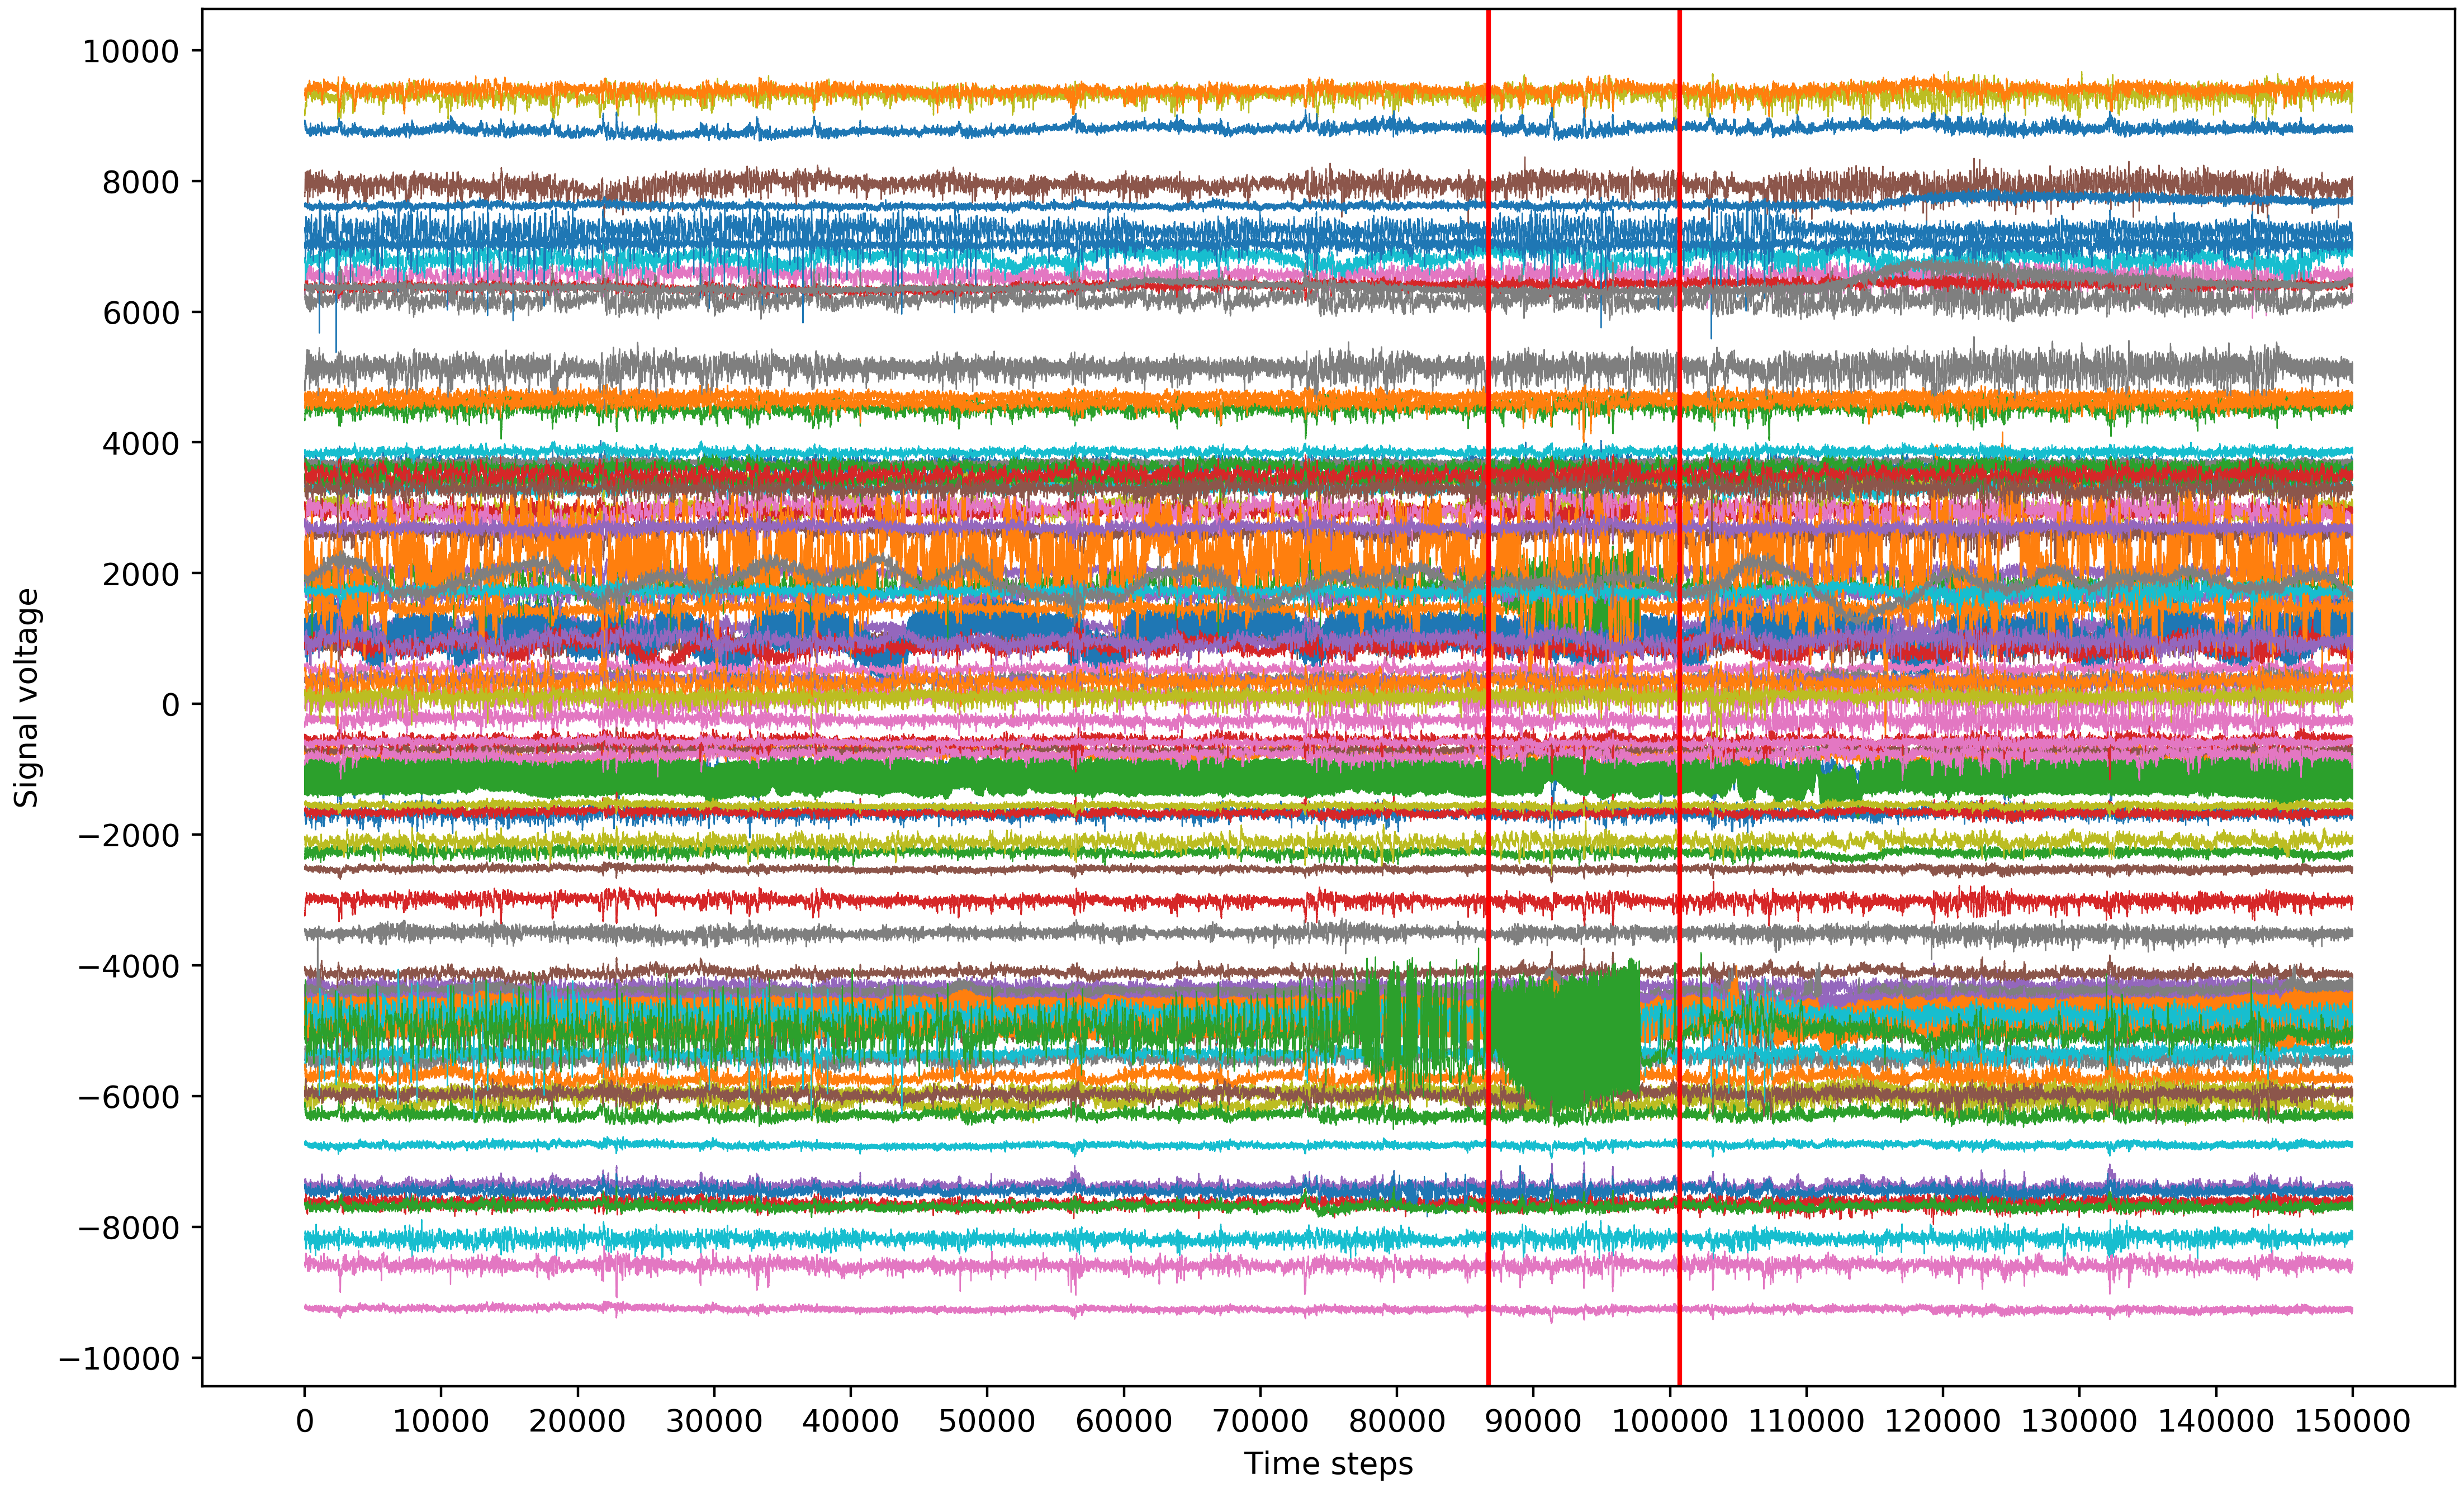
\includegraphics[width=1\textwidth]{plot_seizure3}
        \caption{Third epileptic seizure}
        \label{fig:plot_seizure3}
	\end{subfigure}
    \caption{Plots of the \acs{ieeg} around the three epileptic seizures (we suggest to zoom-in the figures in the pdf file)}
    \label{fig:plot_seizures}
\end{figure}
\newpage

Looking at Figure \ref{fig:plot_seizures}, it seems like the \acsp{ieeg} is not able to explicitly show the presence of a seizure, since the dynamic of the electrodes signals doesn't seem to undergo a big change in correspondence of the beginning of a seizure. This behaviour suggests that the seizure could not be directly represented by the dynamic of the signals, but it could be represented by the non-linear relations between the electrodes signal's dynamic through time.

The amount of positive time steps, that are the ones inside the seizure portions, corresponds only to the $9.3$\% of the data, with the remaining $90.7$\% of data being negative time steps; therefore we are dealing with very unbalanced data (see Figure \ref{fig:hist_classes}). The extreme unbalance of the data, together with the severe restriction in the amount of data, make this dataset very difficult to work with, but at the same time very similar to a real-world scenario.
\begin{figure}[htbp]
    \centering
    \includegraphics[width=0.6\textwidth]{hist_classes}
    \caption{Histogram of the number of time step for each class}
    \label{fig:hist_classes}
\end{figure}

In order to have an idea of the linear relation between electrodes values, we computed the Pearson correlation coefficient on two sequences of 5 seconds each, one of negative time steps and the other of positive time steps. In Figure \ref{fig:corr_heatmaps} we show the related correlation heatmaps. As you can see from the figures, the correlation heatmap related to the positive time steps reveals a higher linear relation between electrodes values if compared to the correlation heatmap related to the negative time steps. The correlation heatmaps, however, present only the linear relations between data, while we believe that there are hidden non-linear relation between electrodes signal through time which could be crucial for the identification of epileptic seizures.

\begin{figure}[htbp]
    \centering
    \begin{subfigure}[t]{0.5\textwidth}
		\includegraphics[width=1\textwidth]{corr_nonseizure}
        \caption{Correlation heatmap of 5 seconds of negative time steps}
        \label{fig:corr_nonseizure}
	\end{subfigure}%
	~
	\begin{subfigure}[t]{0.5\textwidth}
		\includegraphics[width=1\textwidth]{corr_seizure}
        \caption{Correlation heatmap of 5 seconds of positive time steps}
        \label{fig:corr_seizure}
    \end{subfigure}
    \caption{Comparison of correlation heatmaps related to negative and positive time steps}
    \label{fig:corr_heatmaps}
\end{figure}

To have another confirm of the presence of some linear relation between electrodes signals, we computed the standard deviation of the oscillation of each electrode, but this time we computed the mean of the standard deviation both over the negative time steps and over the positive ones. The average standard deviation of the oscillation of each electrode over the negative time steps was around 80 \acs{nv}, while the one over the positive time steps was around 93 \acs{nv}. This shows that, during an epileptic seizure, electrodes signals tends to have wider fluctuation margins, but the difference from the standard fluctuation margins doesn't seems to be enough to identify a seizure.







%----------------------------------------------------------------
% Data preprocessing
%----------------------------------------------------------------

\section{Data preprocessing} \label{sec: data_preprocessing}

\subsection{Time steps as samples}
\subsection{Sequences of time steps as samples}
\subsection{Sequences of graphs as samples}
\subsection{Cross-validation}

%----------------------------------------------------------------
% Experiments
%----------------------------------------------------------------

\section{Experiments} \label{sec: experiments}

\subsection{Support Vector Machine experiments}
\subsection{Random forest experiments}
\subsection{Gradient boosting experiments}
\subsection{Dense neural network experiments}
\subsection{Convolutional neural network experiments}
\subsection{LSTM neural network experiments}
\subsection{Graph-based LSTM neural network experiments}
\subsection{Graph-based convolutional neural network experiments}


%----------------------------------------------------------------
% Results
%----------------------------------------------------------------

\section{Results} \label{sec: results}

\subsection{Experiments results}

